\section{Object Detection}
\label{sec:ObjectDetection}

Since the topic of this thesis concerns the task of \emph{visual} object tracking, an indispensable step in the processing pipeline will unquestionably be object detection. Here we give an overview of various types of image inference to highlight the importance of object detection. The general task of image inference comes in three types, where each builds upon the previous one. The dependency chain is the following: \emph{object classification} $\to$ \emph{object detection} $\to$ \emph{image segmentation}. Due to length constraints for this document, we will focus on object detection as it is the most important of the three for \gls{vot}. We do admit that the object detection strongly relies upon classification because the object cannot be localized (bound) without classifying it.

Object detection comes in various types discussed in the following sections. For our purposes, we will focus on applying the current \gls{sota} techniques with no intention of significantly contributing to object detection methods themselves. Nevertheless, we will put a great emphasis on the performance of the chosen algorithm, since faulty detection with high confidence can hardly be corrected later on. From a holistic point of view, there are \emph{fast} object detectors, such as the most prominent one, \gls{yolo}~\cite{redmon2016yolo} (section~\ref{ssec:YouLookOnlyOnce}), or \gls{ssd}~\cite{liu2016ssd}. Here we use the term \emph{fast} to denote that the detector can operate on high \gls{fps}. This comes at a cost of relatively lower accuracy, though, as compared to \emph{slower} but more accurate approaches based on region proposals, such as various versions of \fasterrcnn{} (section \ref{ssec:FasterRCNN}).

Historically speaking, object detection in its early stages of development depended on feature engineering followed by some shallow machine learning model (e.g. \gls{svm}~\cite{cortes1995support}) to classify the proposed object. Feature extraction was achieved using approaches such as \gls{sift}~\cite{lowel1999objrecognition}, an algorithm capable of producing description of local features in images. Another eminent approach was \gls{hog}~\cite{mcconnell1986osti}, equally used for feature extraction by taking advantage of a change in orientation of gradients in localized portions of the image and subsequently counting occurrences of various orientations. But, as we stated, robust object detection is what our task demands, and the goal of getting the top performance is unattainable without deep learning-based object detection, the principal topic of this section.

Object detection is by its very nature a difficult task, because the number of objects is unknown in advance, which means, that the number of outputs of the model is variable. In terms of a standard deep learning model as described in section~\ref{ssec:ArtificialNeuralNetworks}, this represents a nuisance. A plethora of attempts have been proposed to evade this inherent shortage of standard neural networks. An obvious solution is to only produce a constant number of \glspl{bbox}, as utilized by \gls{ssd} and \gls{yolo}, for instance. But methods based on region proposals try to circumvent the obstacle of having to predict only a fixed set of \glspl{bbox}. Other differences between object detectors stem from the architecture itself, whether the training is an end-to-end pipeline or the model consists of various parts. Fully convolutional architectures are also becoming more prevalent and the latest results are promising~\cite{tian2019fcos}. We will also review fully convolutional trackers in great detail in section \ref{ssec:FullyConvolutionalTracking}.

% ##############################################################################
\subsection{Non-Maximum Suppression}
\label{ssec:NonMaximumSuppression}

Before we dive into the description of the detection itself, we first introduce a general post-processing approach for test phase inference of an object detector. A typical object detection pipeline employs a region proposal step for object classification. Object detectors have hugely profited from the so-called end-to-end learning paradigm in which proposals, features, and the classifier become part of one neural network model~\cite{hosang2017learningnms}. A proposal, in this setting, is nothing but a region containing a potential object of interest. However, the number of proposals may grow considerably, outnumbering the real count of present objects of interest. Moreover, these proposals may have a large overlapping region as measured by \gls{iou} (section \ref{eq:IntersectionOverUnion}), rendering most of them useless in terms of conveying new information, as the majority could cover pretty much the same region. To filter such proposals and extract only the relevant ones, the \gls{nms} algorithm introduced below is used (see \figstr{}~\ref{fig:NonMaximumSuppression}). This post-processing algorithm is responsible for uniting all detected \glspl{bbox} belonging to the same object~\cite{hosang2017learningnms}.

The central idea is to iteratively select only region proposals the \gls{iou} of which is below a specific threshold, i.e. the area they share does not exceed a particular value. But the search for proposals is executed with respect to their confidence level (detection score), since regions produced with higher score should be preserved first. Another reason to evade the occurrence of false positives with high confidence during the detection as much as possible.

For a more formal description, let $\mset{B} = \cbrackets{\vect{b}_1, \vect{b}_2, \dots, \vect{b}_n}$ be a set of $n$ region proposals described by $n$ \glspl{bbox}. Scores for each detection are contained in a set $\mset{S} = \cbrackets{s_1, s_2, \dots, s_n}$, where $s_i$ denotes a detection score for the $i$-th box, $\vect{b_i}$. Let $\lambda$, such that $0 \leq \lambda < 1$, denote a threshold for the maximum allowed portion of the overlap between regions. $\mset{B}_{nms}$ is the set of filtered proposal instances from the set $\mset{B}$ produced using the \gls{nms} algorithm below (inspired by~\cite{bodla2017softnms}):

\begin{algorithmic}[1]
    \Function{NMS}{$\mset{B}$, $\mset{S}$, $\lambda$}

    \State $\mset{B}_{nms}$ $\gets$ $\emptyset$
    \Comment{initialize the output (filtered) set of region proposals}

    \While {$\mset{B} \neq \emptyset$}
    \Comment{loop until all the proposals are processed}

    \State $m \gets \underset{i \in \cbrackets{1, 2, \dots, \msetsize{S}}}{\argmax{}} \mset{S}$
    \Comment{find an index of a proposal with the highest score}

    \State $\mset{B} \gets \mset{B} - \vect{b}_m$, $\mset{S} \gets \mset{S} - s_m$
    \Comment{remove the proposal}

    \State $\mset{B}_{nms} \gets \mset{B}_{nms} \cup \vect{b_m}$
    \Comment{save the proposal with the highest score}

    \For{$i \gets 1$ to $\msetsize{B}$}
    \Comment{iterate through remaining proposals}

    \If{\Call{iou}{$\vect{b}_m$, $\vect{b}_i$} $\geq \lambda$}
    \Comment{\gls{iou} (equation~\ref{eq:IntersectionOverUnion}) exceeds the threshold}

    \State $\mset{B} \gets \mset{B} - \vect{b}_i$, $\mset{S} \gets \mset{S} - s_i$
    \Comment{remove the proposal}
    \EndIf
    \EndFor
    \EndWhile

    \State \Return $\mset{B}_{nms}$
    \EndFunction
\end{algorithmic}

\begin{figure}[t]
    \centerline{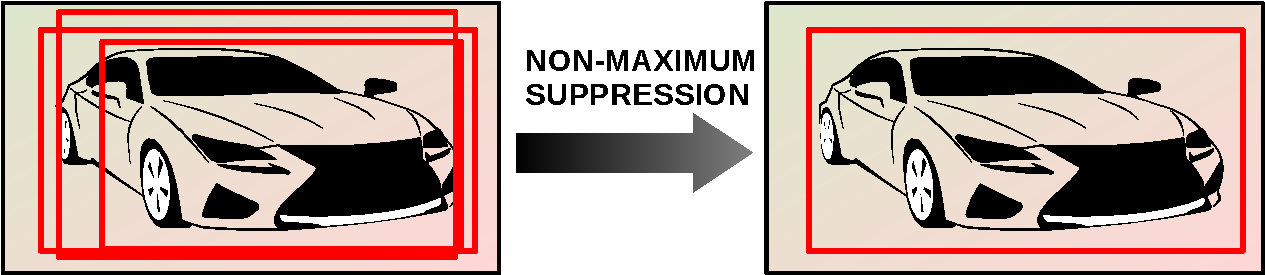
\includegraphics[width=0.7\linewidth]{figures/theoretical_foundations/non_maximum_suppression.pdf}}
    \caption[\Gls{nms} visualization]{An illustration of a potential effect of the \gls{nms} algorithm on \glspl{bbox}. Multiple proposals (left) are filtered so that only the ones with the highest detection score (right) remain while satisfying the condition that the overlap does not exceed a specific threshold.}
    \label{fig:NonMaximumSuppression}
\end{figure}

% ##############################################################################
\subsection{YOLO}
\label{ssec:YouLookOnlyOnce}

\Gls{yolo} is a very popular object detector thanks to its ability to run in real-time and yet be very accurate. Its speed is primarily a consequence that \emph{it looks only once} at a given input image. Compared to region proposal-based approaches, where each object proposal has to be classified separately, resulting in multiple inferences by a potentially huge neural network model, the authors of \gls{yolo} devised a \gls{cnn} model capable of performing extraction of region proposals as well as classification in a single run~\cite{redmon2016yolo}. Besides, the backbone \gls{cnn} model responsible for handling the visual input processes an entire image during the training and test time, allowing the implicit inclusion of contextual information about classes together with their visual representation. During the testing phase, after the single forward propagation through the neural network is executed, the \gls{nms} algorithm is employed to filter predictions to make sure that each object instance is detected just once. It is needless to say that \Gls{yolo} performs well at learning representations that make the generalization easier, which makes this approach well suited for a general object detector, as long as it has been trained on the target domain~\cite{redmon2016yolo}. Since the initial introduction of this approach~\cite{redmon2016yolo}, multiple updates have been brought forward, either from the main author himself~\cite{redmon2017yolo9000, redmon2018yolov3}, or from other researchers~\cite{wang2020yolov4, wong2019yolonano}. Such an interest supports the assertion that \gls{yolo} has great potential for further research as well as real-world applications. In our work, it is a prominent candidate for an object detector that we would train specifically for detecting vehicles and become a part of the object tracking pipeline.

The main implementation aspect is the unification of separate components of object detection into a single neural network. Training is thus executed in an end-to-end fashion. In the original article~\cite{redmon2016yolo}, the model was pre-trained on ImageNet~\cite{deng2009imagenet} classification task at half the resolution of $224 \times 224$. When detecting, the resolution was doubled to get required $448 \times 448$ (\figstr{}~\ref{fig:YOLOGeneralIdea}). The network uses features from the entire image for the prediction of each \gls{bbox}. It also simultaneously predicts all \glspl{bbox} across all classes~\cite{redmon2016yolo}.

As shown in \figstr{}~\ref{fig:YOLOBBOXESProgression}, the input image is divided into an $S \times S$ grid. Since most of the time an object will overlap multiple grid cells, the \emph{main} cell responsible for predicting the object will be the one the center of the object's \gls{bbox} falls into. Each \gls{bbox} prediction is evaluated by a confidence level computed as $\prob{\text{object}} \cdot \func{IOU}{\vect{b}_{pred}, \vect{b}_{truth}}$, with $\vect{b}_{pred}$ and $\vect{b}_{truth}$ being the prediction and ground truth, respectively. If no object exists in a particular cell, the confidence should be equal to $0$. Each grid cell prediction also encapsulates $C$ conditional probabilities for each class under the assumption that the object is present, mathematically stated as $\probgiven{{\text{class}}_i}{\text{object}}$. But only one set of class probabilities is predicted per grid cell, regardless of the value of the hyperparameter $B$. This description can be concisely conveyed by the equation below:
\begin{equation}
    \begin{aligned}
        \label{eq:YOLOCOnfidenceScores}
         & \probgiven{{\text{class}}_i}{\text{object}}
        \cdot
        \prob{\text{object}}
        \cdot
        \func{IOU}{\vect{b}_{pred}, \vect{b}_{truth}}
        =                                              \\
         & \prob{{\text{class}}_i}
        \cdot
        \func{IOU}{\vect{b}_{pred}, \vect{b}_{truth}}.
    \end{aligned}
\end{equation}
This equality gives the class-specific confidence score which basically encodes both the probability of the $i$-th class appearing in a particular \gls{bbox} in conjunction with how well this predicted box fits the object.

\begin{figure}[t]
    \centerline{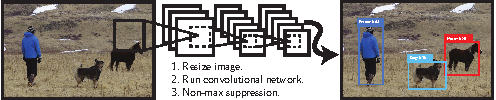
\includegraphics[width=0.8\linewidth]{figures/theoretical_foundations/yolo_general_idea.pdf}}
    \caption[\Gls{yolo} processing pipeline]{Processing of images using \gls{yolo} requires the input image to have the resolution of $448 \times 448$ pixels. Then, a single run of the convolutional network happens, followed by the thresholding of the resulting detections according to their confidence. \externalsrc{\cite{redmon2016yolo}}}
    \label{fig:YOLOGeneralIdea}
\end{figure}

\begin{figure}[t]
    \centerline{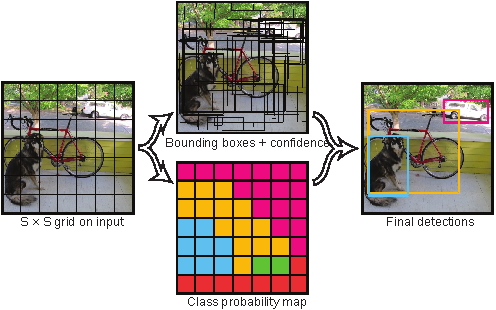
\includegraphics[width=0.8\linewidth]{figures/theoretical_foundations/yolo_bboxes_progression.pdf}}
    \caption[\Gls{yolo} detections]{This model treats detections as a regression problem. The image is divided into $S \times S$ grids, for each grid $B$ \glspl{bbox} are predicted with associated confidence, and for each box $C$ class probabilities are inferred. The prediction tensor has therefore size of $S^2 \times \rbrackets{5B + C}$. \externalsrc{\cite{redmon2016yolo}}}
    \label{fig:YOLOBBOXESProgression}
\end{figure}

The network design reflects a standard practice in deep learning-based computer vision model, where a \gls{cnn} backbone is used to extract features followed by fully connected layers. In this case, the two fully connected layers are in charge of prediction of the output probabilities and coordinates (\figstr{}~\ref{fig:YOLOArchitecture}).

\begin{figure}[t]
    \centerline{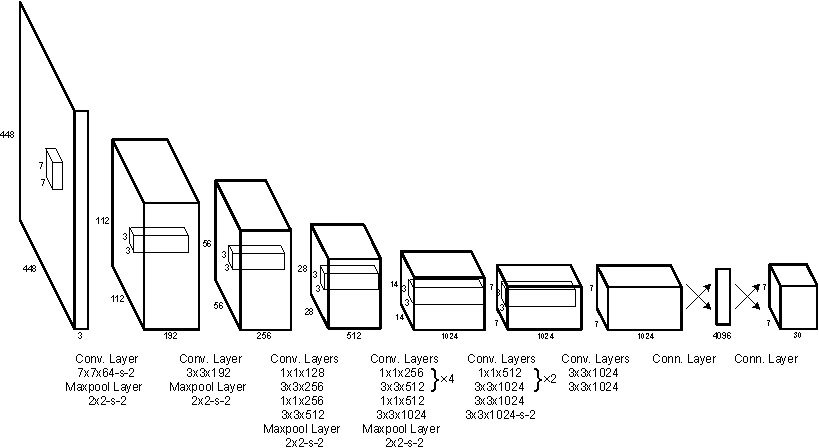
\includegraphics[width=0.8\linewidth]{figures/theoretical_foundations/yolo_architecture.pdf}}
    \caption[\Gls{yolo} architecture]{The \gls{yolo} model architecture consisting of 24 convoutional layers followed by two fully connected layers at the end. The alternation of $1 \times 1$ convolutional layers is used to reduce the feature space size. \externalsrc{\cite{redmon2016yolo}}}
    \label{fig:YOLOArchitecture}
\end{figure}

% ##############################################################################
\subsection{Faster R-CNN}
\label{ssec:FasterRCNN}

Apart from the two already introduced approaches, this one, \fasterrcnn{}, employs \emph{two-stage} object detection. The first stage consists of generating region proposals using the \gls{rpn}~\cite{ren2017fasterrcnn} (\figstr{}~\ref{fig:FasterRCNNRPN}), where the input image is processed by a feature extractor~\cite{huang2017speedacctradeoff}. These class-agnostic proposals, a set of rectangular boxes, are produced from an input of arbitrary size (allowed by the fact that this process is modeled by a fully convolutional network) (\figstr{}~\ref{fig:FasterRCNNMetaArch}).

As far as the second stage is concerned, the proposed regions (usually $300$) serve as a basis for subsequent cropping of features from the same intermediate feature map which are then fed to the remaining feature extractor to predict the class. Based on this class prediction, the proposed box is further refined. The name for this stage is \emph{box classifier}.

\begin{figure}[t]
    \centerline{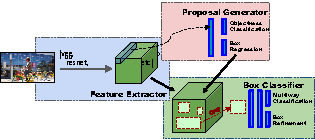
\includegraphics[width=0.7\linewidth]{figures/theoretical_foundations/faster_rcnn_metaarchitecture.pdf}}
    \caption[\fasterrcnn{} meta-architecture]{A meta-architecture of the \fasterrcnn{} model. \externalsrc{\cite{huang2017speedacctradeoff}}}
    \label{fig:FasterRCNNMetaArch}
\end{figure}

As the endeavor is to diminish unnecessary computations, the proposals are not cropped explicitly from the input image, and then processed by the feature extractor. Nevertheless, there is a part of the computation that has to be executed once per each proposed region, so the performance depends on the number of regions generated by the \gls{rpn}.

\begin{figure}[t]
    \centerline{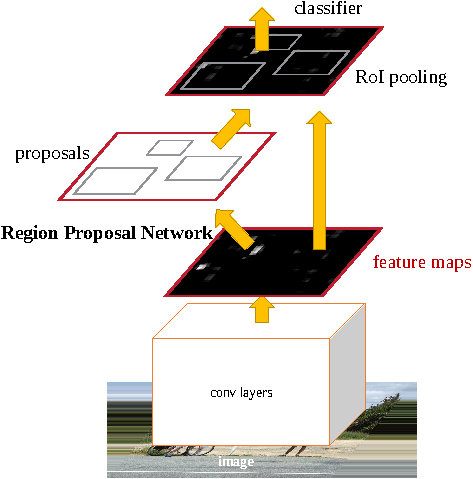
\includegraphics[width=0.5\linewidth]{figures/theoretical_foundations/faster_rcnn_rpn_module.pdf}}
    \caption[\fasterrcnn{} with the \gls{rpn}]{The \fasterrcnn{} is built as a unified network for object detection, with its \gls{rpn} module serving the purpose of an \emph{attention}. \externalsrc{\cite{ren2017fasterrcnn}}}
    \label{fig:FasterRCNNRPN}
\end{figure}

% ##############################################################################
\subsection{Fully Convolutional Object Detection}
\label{ssec:FullyConvolutionalObjectDetection}

\todo[inline]{Emphasize centerness more since SiamMOT exploited it, too. Also mention Siamese architectures that also used it.}

Recent research shows that utilizing fully convolutional networks provides many advantages. Not only the input can be of arbitrary size thanks to the absence of fully connected layers, but the number of hyperparameters is reduced, too. We will now discuss the \gls{fcos} model. This work was inspired by one-stage detectors such as \gls{yolo} and \gls{ssd} and by how semantic segmentation operates on the level of pixels. The proposed solution by~\cite{tian2019fcos} is anchor-free as well as proposal-free. The elimination of anchors avoids complicated computations related to anchor boxes, such as calculating overlapping regions during training. More importantly, anchor boxes come with many initialization-sensitive hyperparameters, namely their number and dimensions.

\Gls{fcos} is built on top of \gls{fpn}~\cite{li2019weightedfpn}, which aggregates features from the backbone at multiple levels, reminiscing a pyramidal shape. Predictions are thereafter obtained across $5$ feature levels from the \gls{fpn} (\figstr{}~\ref{fig:FCOSFeaturePyramid}). \gls{fpn} makes use of the scale-invariant properties of feature pyramids, which enable object detection over a wide range of scales.

Authors came up with a concept of \emph{centerness}, which describes the amount of deviation of the pixel's location from the object center (\figstr{}~\ref{fig:FCOSCenterness}). The reason for adding this score was to suppress locations that are further away from the object's center, because they produced low-quality \gls{bbox} predictions. This score is then used as a weighting factor for the class prediction score. Let $l^*$, $t^*$, $r^*$ and $b^*$ be the regression targets for the box. Then the \emph{centerness} $\func{C}{\cdot}$ is computed as

\begin{equation}
    \label{eq:CenternessDetection}
    \func{C}{l^*, t^*, r^*, b^*} =
    \sqrt{
        \frac{
            \func{\min}{l^*, r^*}
        }{
            \func{\max}{l^*, r^*}
        }
        \times
        \frac{
            \func{\min}{t^*, b^*}
        }{
            \func{\max}{t^*, b^*}
        }
    }.
\end{equation}


\begin{figure}[t]
    \centerline{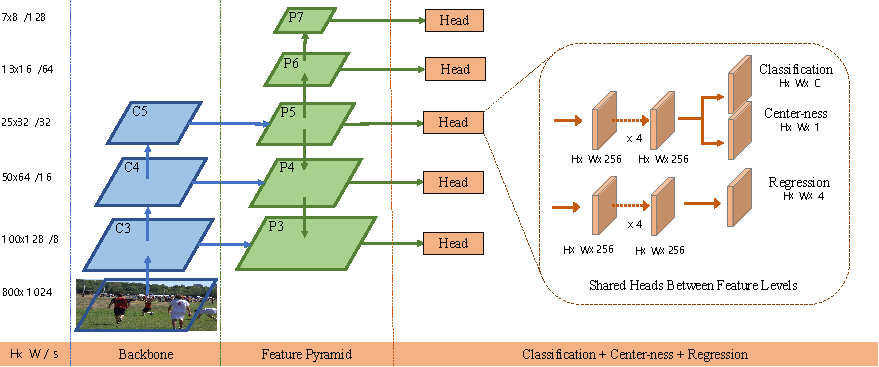
\includegraphics[width=\linewidth]{figures/theoretical_foundations/fcos_feature_pyramid.pdf}}
    \caption[\Gls{fcos} architecture]{The network architecture of the \gls{fcos}. Feature maps denoted by $C3$, $C4$ and $C5$ belong to the backbone network. Features at the levels from $P3$ to $P7$ are used to make final predictions. For each of these feature maps, the shared head computes the classification (foreground/background disrimination), the \emph{centerness} score and \gls{bbox} regression. \externalsrc{\cite{tian2019fcos}}}
    \label{fig:FCOSFeaturePyramid}
\end{figure}

\begin{figure}[t]
    \centerline{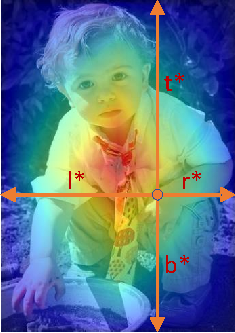
\includegraphics[width=0.25\linewidth]{figures/theoretical_foundations/fcos_centerness.pdf}}
    \caption[Centerness visualization]{Red, blue, and other colors denote $1$, $0$ and the values between them, respectively. Center-ness is calculated as given by eqiation~\ref{eq:CenternessDetection} and decays from $1$ to $0$ as the location deviates from the center of the object. Best viewed in color. \externalsrc{\cite{tian2019fcos}}}
    \label{fig:FCOSCenterness}
\end{figure}

\begin{figure}[t]
    \centerline{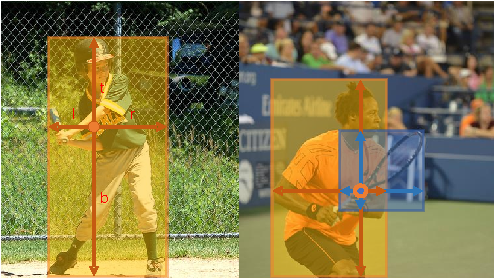
\includegraphics[width=0.6\linewidth]{figures/theoretical_foundations/fcos_detection_demo.pdf}}
    \caption[\Gls{fcos} predictions]{On the left, the model predicts for each pixel in the image a $4D$ vector $\sbrackets{l, t, r, b}^T$ encoding the \gls{bbox} dimensions (supervised by the ground-truth one during the training). On the right, there is a demonstration of possible ambiguity when a pixel resides within more than just one \gls{bbox}. In that case, a decision has to be made which box should be regressed to. \externalsrc{\cite{tian2019fcos}}}
    \label{fig:FCOSDetectionDemo}
\end{figure}
